\documentclass[12pt]{report}
\usepackage{amsmath}
\usepackage{verbatim} 
\usepackage{graphicx}
\usepackage{algorithmicx}
\usepackage{algpseudocode}
\begin{document}
\begin{titlepage}
\title{GDDB \\ Graphical Datalog Debugger}
\author{Jade Koskela\\ \texttt{jtkoskela@ucdavis.edu} \\ \\
Undergraduate Research Supervised by Dr. Bertram Ludaescher\\
Department of Computer Science\\
University of California, Davis
}
\date{Spring 2012}
\maketitle
\end{titlepage}
\section*{Datalog: A Brief Overview}
Datalog is a subset of Prolog used for deductive databases. In this project we have used the Datalog extension DLV. The input to the DLV interpreter consists of rules and facts. Rules define the relationships used to infer, from the input facts, what is in our database. The output from datalog is called the model. For example:  \\
\\
\textbf{Rules:}
\[\text{ dog(X) :- pet(X), obendient(X).} \]
\[\text{ cat(X) :- pet(X), fiesty(X).} \]
\[\text{ Earl(X) :- black(X), cat(X).} \]
\[\text{ Max(X) :- red(X), dog(X).} \] 
\textbf{Facts:} \\
\[\text{ mammal(x).} \]
\[\text{ fiesty(x).} \]
\[\text{ black(x).} \]
\\
This input will generate the output model:\\ \[\emph{\{mammal(x), black(x), fiesty(x), cat(x), Earl(x)\}} \] We have derived the new atoms: \emph{cat(x)} and \emph{Earl(x)}. 

\section*{Debugging}

\subsection*{Derivation Tree}
In a large program we would have many atoms or tuples in our output model. We would like to be able to determine how each atom was derived. GDDB gives us the ability to visually inspect our derivation tree, and trace the provenance of each tuple in the output. Suppose we wanted to know how $Earl(x)$ came to be in our model. In this simple case it is obvious, however in a more complex case there could be many possible rules that were used in the derivation. In order to build the derivation tree, we create auxiliary rules which model the event where a certain rule was used to create a new tuple. The GDDB parser will create the auxiliary rules from the input rules. In our example, the parser would ouput:

\begin{center}
dog(X) :- aux\_dog\_0(X). \\
aux\_dog\_0(X) :- mammal(X), obedient(X). \\
cat(X) :- aux\_cat\_1(X).  \\
aux\_cat\_1(X) :- mammal(X), fiesty(X). \\
Earl(X) :- aux\_Earl\_2(X).\\ 
aux\_Earl\_2(X) :- black(X), cat(X).\\
Max(X) :- aux\_Max\_3(X). \\
aux\_Max\_3(X) :- red(X),dog(X).\\
\end{center} 
We can now feed the new rules and the original facts to DLV. We get the output model :\\
\[\emph{\{mammal(x), obedient(x), black(x), cat(x), aux\_cat\_1(x), Earl(x), aux\_Earl\_2(x)\}}\]
\bigskip \\
We use Graphviz to render the relationships between the tuples. The unlabeled nodes are the auxiliary tuples.\\
\includegraphics[scale=0.75]{g1.jpg} \\
\bigskip \\
\bigskip \\
\section*{GDDB Usage}
We can perform the workflow from the following example by using the gddb script, which launches the GDDB command line interpreter.
\begin{verbatim}
$ ./gddb animal_rules animal_facts
$ (Cmd) draw
\end{verbatim}
\subsection*{Trace}
In a large graph it maybe difficult to see the derivation of any particular tuple. For example:
\subsubsection*{Input}
\begin{center}
tc(X,Y) :- e(X,Y). \\
tc(X,Y) :- e(X,Z), tc(Z,Y).\\
e(1,2). \\
e(2,3). \\
e(3,4). \\
e(4,5). \\ 
e(4,2). \\
\end{center}
\subsubsection*{Output}
\includegraphics[scale=0.6]{transitive_closure.pdf} \\
\subsubsection*{Trace}
As you can see, the complexity of our graph increases rapidly. To make the derivation of a particular tuple clear, we can trace the provenance by doing a depth first search backwards, up the tree, starting from the tuple traced.
\begin{verbatim}
$ ./gddb tc_rules tc_facts
$ (Cmd) trace tc(4,4)
$ (Cmd) draw
\end{verbatim}
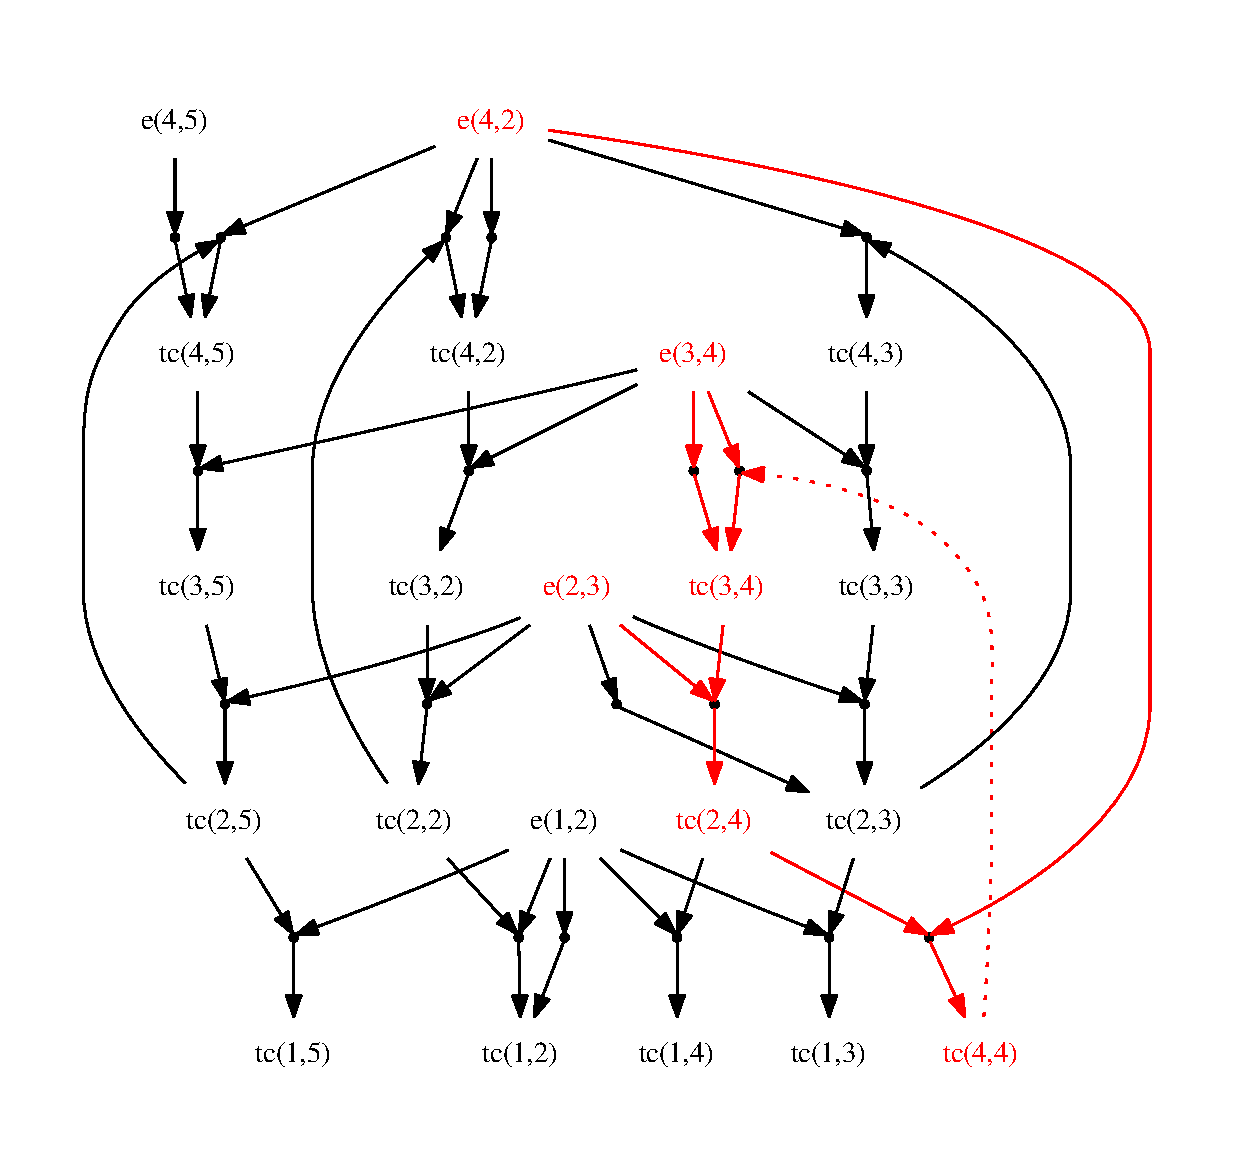
\includegraphics[scale=0.5]{tc_trace_full.pdf} \\
The dashed edges represent backedges, or cycles, in the graph. \\
\bigskip \\
\subsubsection*{Partial Trace}
We can also restrict our trace to only render the tuples which were traversed.
\includegraphics[scale=0.5]{tc_part.pdf} \\
\subsubsection*{Styles}
We can add graphviz styles from an external style sheet.
\begin{verbatim}

negation_out.edges:          {style=dashed, color=red}               
negation_in.edges:           {style=dashed, color=green}               
aux.nodes:                   {shape=point}
root.nodes:                  {shape=plaintext}
root.graph                   {rankdir=LR}


$ ./gddb rel_div_rules rel_div_facts styles
$ (Cmd) draw
\end{verbatim}
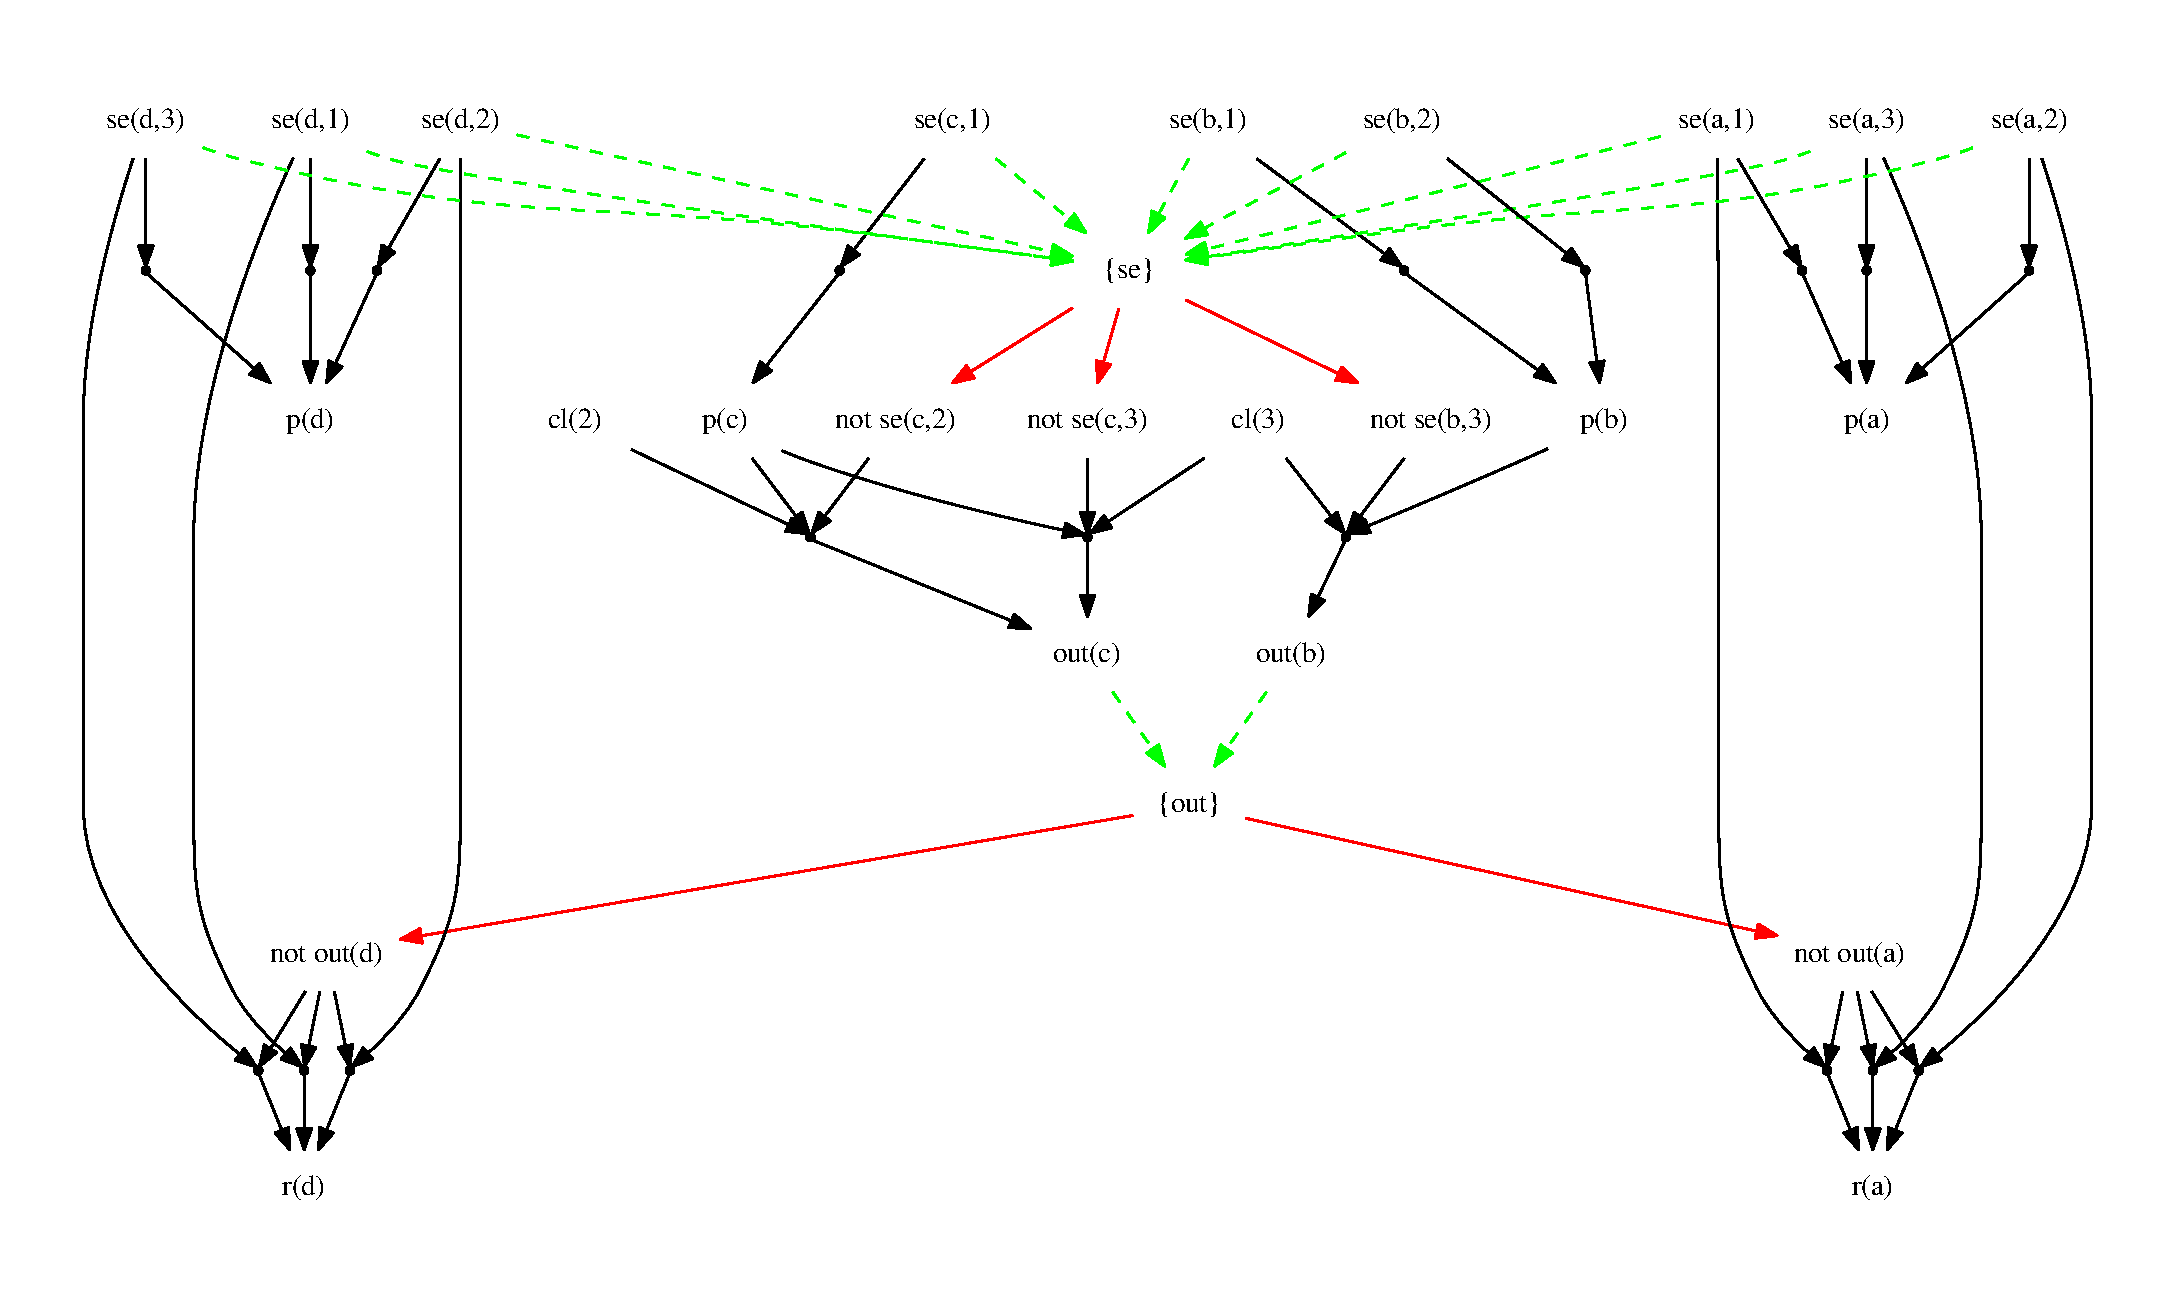
\includegraphics[scale=0.45]{relation_division.pdf} \\
\bigskip \\
\bigskip \\
\\
\\
We can also add styles from the GDDB interpreter.
\begin{verbatim}
$ ./gddb animal_rules animal_facts
$ (Cmd) help set
(Cmd) help set
Set attribute of the graph or subgraphs.
Usage: set [subgraph] [edges|nodes] [attribute] [value]

(Cmd) set root edges color blue
(Cmd) set root nodes shape circle
(Cmd) set root graph rankdir LR
(Cmd) draw
\end{verbatim}
\includegraphics[scale=0.45]{g2.jpg} \\
\end{document}